


\chapter{Informations supplémentaires pour le chapitre \ref{article}} 



\noindent \textit{Evolutionary Applications} Supporting Information for:
\bigskip
\bigskip

\noindent  \textbf{Multiseasonal modelling of plant-nematode interactions  reveals efficient plant resistance deployment strategies}
\bigskip

\noindent Samuel Nilusmas$^1$, Mathilde Mercat$^1$, Thomas
Perrot$^1$, Caroline Djian-Caporalino$^1$,
Philippe Castagnone-Sereno$^1$, Suzanne Touzeau$^{1,2,*}$, Vincent
Calcagno$^{1,*}$,  and Ludovic Mailleret$^{1,2,*}$
\bigskip

\noindent{\footnotesize $^1$Université Côte d'Azur, INRAE, CNRS, ISA, France;\\
$^2$Université Côte d'Azur, Inria, INRAE, CNRS, Sorbonne Université,
BIOCORE, France \\[1ex]
$^*$These authors should be considered joint senior author.}
\bigskip

\noindent
{\small April 2020}
\bigskip

%\vspace{3\baselineskip}

  
\noindent The following Supporting Information is available for this article:

\begin{description}
\item[Fig. S1 ] Diagram representing the plant-nematode interaction
  model for two successive cropping seasons of resistant and
  susceptible plants.

\item[Fig. S2 ] Ratio of resistant plants as a function of the time
  horizon, for different deployment strategies: susceptible-only,
  resistant-only, optimal periodic rotation and optimal unconstrained
  (average value and range).

\item[Fig. S3 (within Methods S3)] Global sensitivity indices on
  the healthy root density (a yield proxy) for the optimal periodic rotation
  strategy over a 15-season time horizon.

\item[Methods S1] Computation of the season-to-season basic
  reproduction numbers $R_0$ for avirulent and virulent nematodes.

\item[Methods S2] Model fitting to experimental data describing the
  infection dynamics of susceptible tomato roots by avirulent
  nematodes during a cropping season.
    
\item[Methods S3] Sensitivity analysis to assess the parameter
    impact on the healthy root density (a yield proxy) for a susceptible-only
  strategy over a 15-season time horizon. 
\end{description}


\begin{figure}[p]
  \centering
  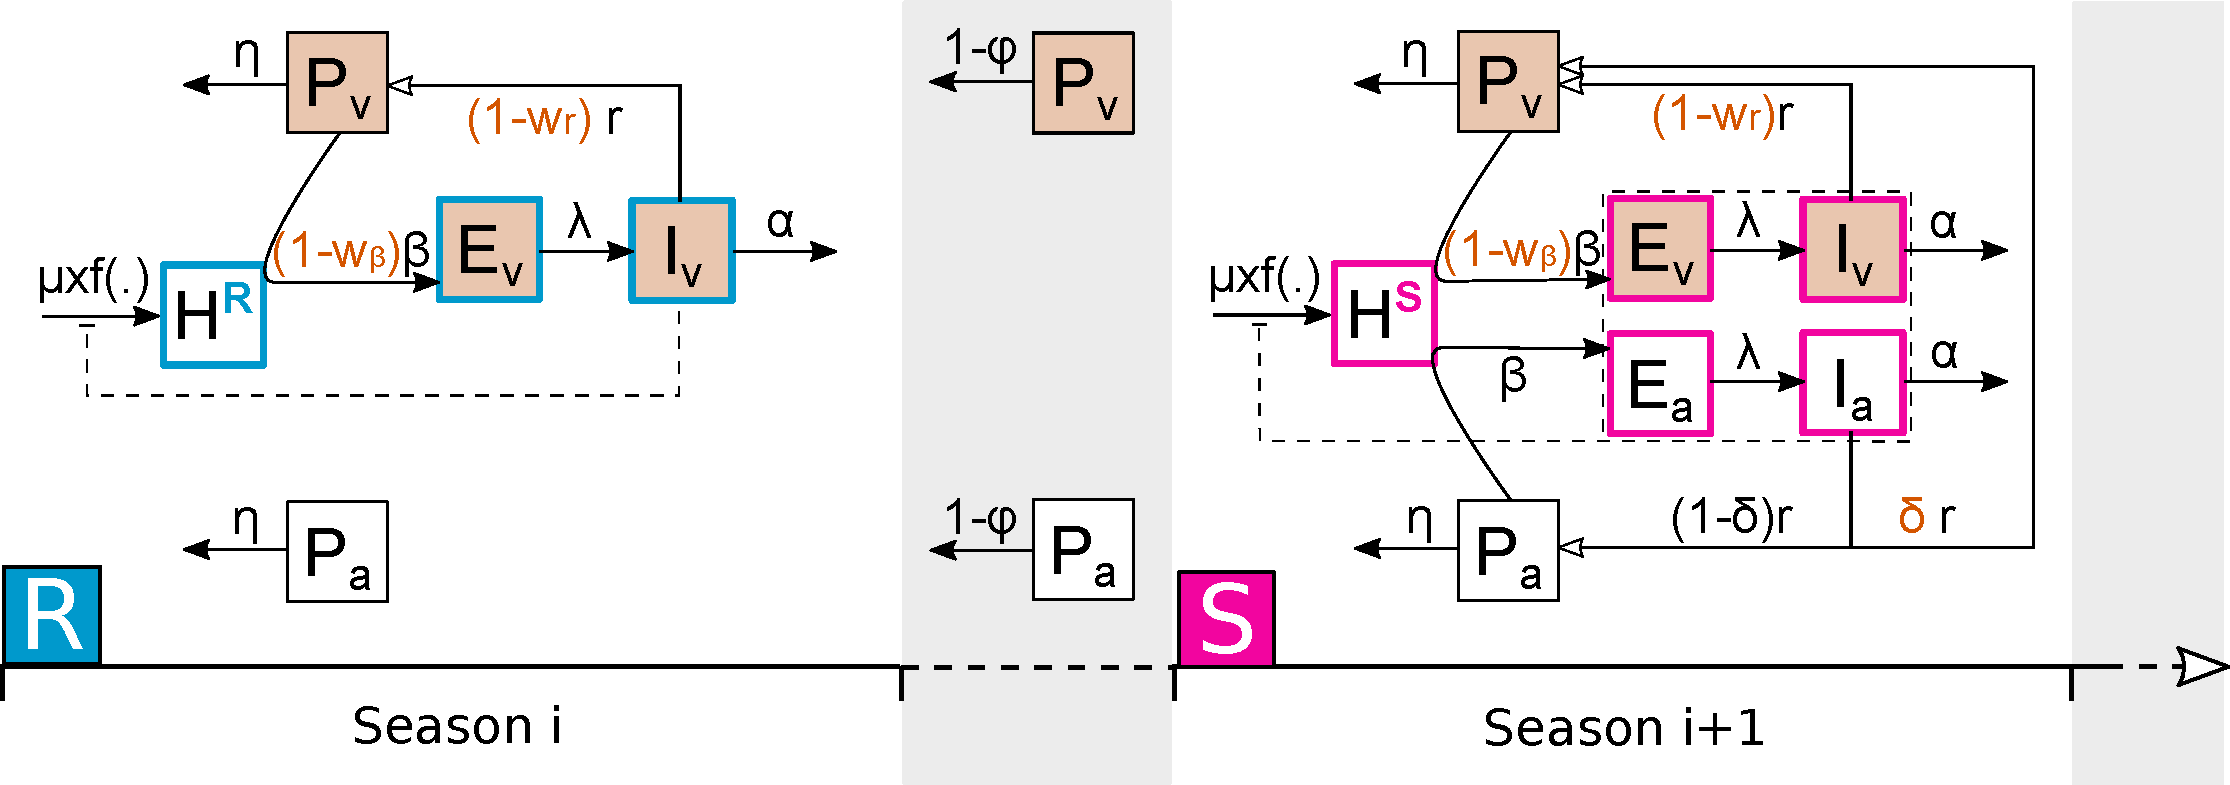
\includegraphics[width=\linewidth]{figS1.pdf}
  \caption[Plant-nematode interaction model for two successive cropping
    seasons of resistant  and susceptible
    plants]{Compartmental diagram representing the
    plant-nematode interaction model for two successive cropping
    seasons of resistant (superscript $X=R$) and susceptible
    (superscript $X=S$) plants. Healthy plant roots ($H^X$) are
    infected by virulent (subscript $v$) and avirulent (subscript $a$)
    nematodes in the soil ($P$), before becoming latently infected
    ($E=E_a +E_v$) and then infectious ($I=I_a + I_v$) feeding
    sites. Between cropping seasons (shaded area), free living
      nematodes remain in the soil. Parameters are described in Table~1 (main text).}
  \label{figS1}
\end{figure}

\begin{figure}[p]
  \centering
  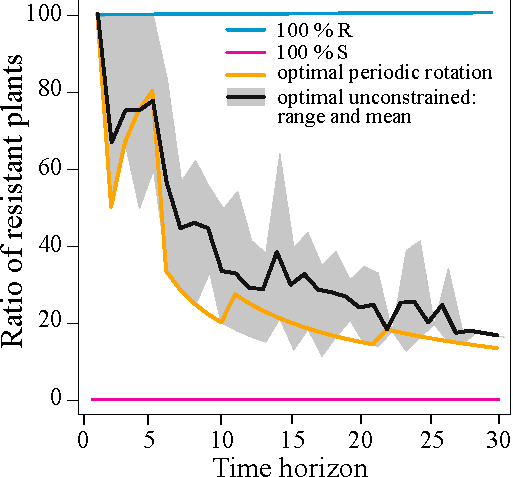
\includegraphics[width=.5\linewidth]{figS2.pdf}
  \caption[Ratio of resistant plants as a function of the time
    horizon, for different deployment strategies]{Ratio of resistant plants as a function of the time
    horizon, for different deployment strategies: susceptible-only
    (pink), resistant-only (blue), optimal periodic rotation (yellow)
    and optimal unconstrained (black). Different unconstrained optimal
    strategies (yielding the same $\overline{HRD}$) were identified,
    so the ratio is represented by its range (shaded area) and its
    average value (black solid curve). Default parameter values were
    used (Table~1 in main text).}
  \label{figS2}
\end{figure}



\clearpage
\section{Methods S1. Computation of the season-to-season basic reproduction numbers $R_0$} 

Season-to-season basic reproduction numbers quantify the multiplication rate of a pathogen from the beginning of a cropping season to the beginning of the next season, when pathogen densities are vanishingly low\footnote{Mailleret, L., Castel, M., Montarry, J., Hamelin, F. M. (2012). From elaborate to compact seasonal plant epidemic models and back: Is competitive exclusion in the details? \emph{Theoretical Ecology}, 5, 311--324.}.

To evaluate the basic reproduction number of avirulent nematodes $P_a$ on susceptible plants, we assumed that the dynamics of infected feeding sites $E_a$ and $I_a$ were fast and that the fraction of virulent  offspring $\delta$ tended to 0. Under these approximations, the dynamics of free living nematodes $P_a$ becomes:
\begin{equation*}
\dot{P}_a(t)=P_a(t) \left(  \beta\left( \frac{ \epsilon_a^S r}{\alpha}-1\right) H^S(t) - \eta \right),
\end{equation*}
so that:
\begin{equation*}
  P_a (\tau)= \exp\left(\int_{t=0}^{t=\tau} \left(\beta\left(\frac{ \epsilon_a^S r}{\alpha}-1\right) H^S(t)  - \eta\right) dt\right)P_a(0).
\end{equation*}
Healthy roots  grow linearly in the absence of nematodes so that at time $t$ during the course of a season $H^S(t) = H_0 + \mu x t$. Therefore:
\begin{equation*}
  P_a(\tau) = \exp\left(\beta\left( \frac{\epsilon_a^S r}{\alpha}-1\right) \left( H_0 \tau+\frac{\mu x \tau^2}{2}\right)-\eta \tau\right)P_a(0).
\end{equation*}
Taking into account between-season survival $\varphi$, the season-to-season basic reproduction number of avirulent nematodes on susceptible plants therefore reads:
\begin{equation*}
  R_{0,a}^S= \varphi \exp\left(\beta\left( \frac{\epsilon_a^S r}{\alpha}-1\right) \left( H_0 \tau+\frac{\mu x \tau^2}{2}\right)-\eta \tau\right).
\end{equation*}

One can proceed in a very same way to compute the basic reproduction number of avirulent nematodes on resistant plants, accounting for the absence of free living nematodes produced during such a season. This yields:
\begin{equation*}
  R_{0,a}^R= \varphi \exp\left(-\beta \left( H_0 \tau+\frac{\mu x \tau^2}{2}\right)-\eta \tau\right),
\end{equation*}
which is clearly lower than $1$.

Finally, since virulent nematodes develop similarly on resistant and susceptible plants, their basic reproduction number is the same on both plants. Applying the method described above and taking into account the presence of fitness costs $w_\beta$ and $w_r$, this leads to:
\begin{equation}
R_{0,v} = \varphi \exp\left(\beta\left( \frac{(1-w_\beta)(1-w_r)\epsilon_v r}{\alpha}-1\right) \left( H_0 \tau+\frac{\mu x \tau^2}{2}\right)-\eta \tau\right). \label{R0v}
 \end{equation}
Introducing the effective fitness cost $w^*=1-(1-w_\beta)(1-w_r)$, one gets:
\begin{equation*}
  R_{0,v} = \varphi \exp\left(\beta\left( \frac{(1-w^*)\epsilon_v r}{\alpha}-1\right) \left( H_0 \tau+\frac{\mu x \tau^2}{2}\right)-\eta \tau\right).
\end{equation*}


\clearpage
\section{Methods S2. Model fitting to experimental data} \label{MethodsS2}

Three parameters could not be set from published data: the infection rate ($\beta$), the conversion factor between root biomass and density of feeding sites ($x$) and the plant
growth scaling factor ($k$). To estimate these parameters, data obtained by Ehwaeti \textit{et al.}\footnote{Ehwaeti, M. E., Phillips, M. S., Trudgill, D. L. (1998). Dynamics of damage to tomato by Meloidogyne incognita. \emph{Fundamental and Applied Nematology}, 21(5), 627–635.} were used. They describe the infection dynamics of susceptible tomato (cv \textit{Moneymaker}) roots by avirulent  nematodes \textit{Meloidogyne incognita}, which were initially inoculated in the soil at five controlled densities ($P_0(i)$ with $i=1,\ldots,5$). The nematode density in the roots  ($N_\text{data}$) was measured after 42 days and 135 days of cultivation. The relative root biomass ($B_\text{data}$), \textit{i.e.}\ the root biomass  of an infected plant divided by the root biomass of an uninfected plant, was also measured. Both measures were reported as a mean over five replicates, for each initial nematode density. Only final measures after 135 days of cultivation were used to estimate the parameters (measures after 42 days were used to assess the model validity).

Model fitting was performed by finding the  $x, k, \beta$ and $y$ parameter values that minimised the distance between the model output and the data using on a weighted square metric:
\begin{equation*}
J(x,k,\beta) = \sum_{i=1}^{5} \left(\dfrac{N_\text{model}(i,x,k,\beta) -N_\text{data}(i)}{\text{mean}_i(N_\text{data}(i))} \right)^2 
+\sum_{i=1}^{5}  \left(\dfrac{B_\text{model}(i,x,k,\beta,y) -B_\text{data}(i)}{\text{mean}_i(B_\text{data}(i))} \right)^2.
\end{equation*}
Parameter $y$ was introduced to take into account the extra root mass corresponding to the root-knot galls caused by nematodes. It was estimated along with the three other parameters. $N_\text{model}(i,x,k,\beta)$ and $B_\text{model}(i,x,k,\beta)$ were computed, based on model~(Eqn~3.1, main text) integrated at time $t=135$ days, as follows:
\begin{align*}
  N_\text{model}(i,x,k,\beta)&= E_a(135)+I_a(135),\\
  B_\text{model}(i,x,k,\beta,y)&= \frac{H^S(135)+y\,E_a(135)+y\,I_a(135)}{H^{S*}(135)},
\end{align*}
with the initial nematode density in the soil  $P_a(0)=P_0(i)$, except for $H^{S*}$ which was computed with $P_a(0)=0$, and with given parameters $x,k,\beta$ and $y$ (remaining parameter values can be found in Table~1, main text).

Division by the means made both $N$ and $B$ terms dimensionless so they could be summed. The computation of the parameter values that minimised $J$ was achieved using the optim function of R with the default Nelder-Mead method.


\clearpage
\section{Methods S3. Sensitivity analysis} \label{ans}

We performed a global sensitivity analysis to assess the parameter impact on the healthy root density ($\overline{HRD}$) for the $1R+5S$ optimal periodic rotation strategy over a 15-season time horizon. The method used is based on factorial design and analysis of variance (ANOVA). The $\overline{HRD}$ was considered as the output (or observation), the parameters as factors.

We first explored the parameter space  by varying  all parameters, except the nematode infection success $\epsilon_y^X$ (a Boolean)  and the duration of a cropping season $\tau$. We chose three levels per parameter: the default value found in the literature or estimated according to Supporting Information Methods~S2 and $\pm 30\%$ variations, except for $P_0$ for which larger variations were chosen (Table~1, main text). A full factorial design, defined as all possible combinations of the three parameter levels, corresponds to $3^{14}=4,782,969$ combinations and would have required the same number of simulations to compute the corresponding $\overline{HRD}$. To reduce this number, we implemented a fractional factorial design (a subset of the full design), chosen in order to estimate all parameter main effects  and two-way interactions. The fractional factorial design was obtained using the \textsc{planor} R package (\href{https://CRAN.R-project.org/package=planor}{https://CRAN.R-project.org/package=planor}) and consisted of 2187 parameter combinations, yielding as many simulations.

By means of an ANOVA, we then proceeded with the observed variance decomposition and estimated the sum of squares associated with each factorial term, main effect $SS_i$ or the two-way interaction $SS_{i,j}$. According to the sparsity-of-effects principle, a system is usually dominated by main effects and low order interactions, so neglecting  higher interactions can still provide good estimates. Denoting by  $SS_{T}$ the total sum of squares, the total sensitivity index of parameter $p_i$ is defined as follows:
\begin{equation}
\label{si}
tSI_i=\frac{\overbrace{SS_{i}}^{\text{main effect}}+\overbrace{ \sum_{j\neq i} SS_{i,j}}^{\text{two-way interactions}}}{SS_{T}}.
\end{equation}
It represents the fraction of the output variability explained by parameter $p_f$. 
We used the \textsc{multisensi} R package (\href{https://CRAN.R-project.org/package=multisensi}{https://CRAN.R-project.org/package=multisensi}) for this analysis.

The results of the global sensitivity analysis are shown in \autoref{figS3}. 
Interactions had little impact, so  parameter main effects largely explained the output variability. Parameters that most influenced the $\overline{HRD}$ were 
the infection rate $\beta$ ($tSI_\beta=30\%$ ), the nematode reproduction rate $r$ ($tSI_r=28\%$), as well as the nematode mortality rates in the soil $\eta$ ($tSI_\eta=23\%$) and in the plant $\alpha$ ($tSI_\alpha=18\%$). The other parameters had little impact on the output.

\begin{figure}[ht]
  \centering
  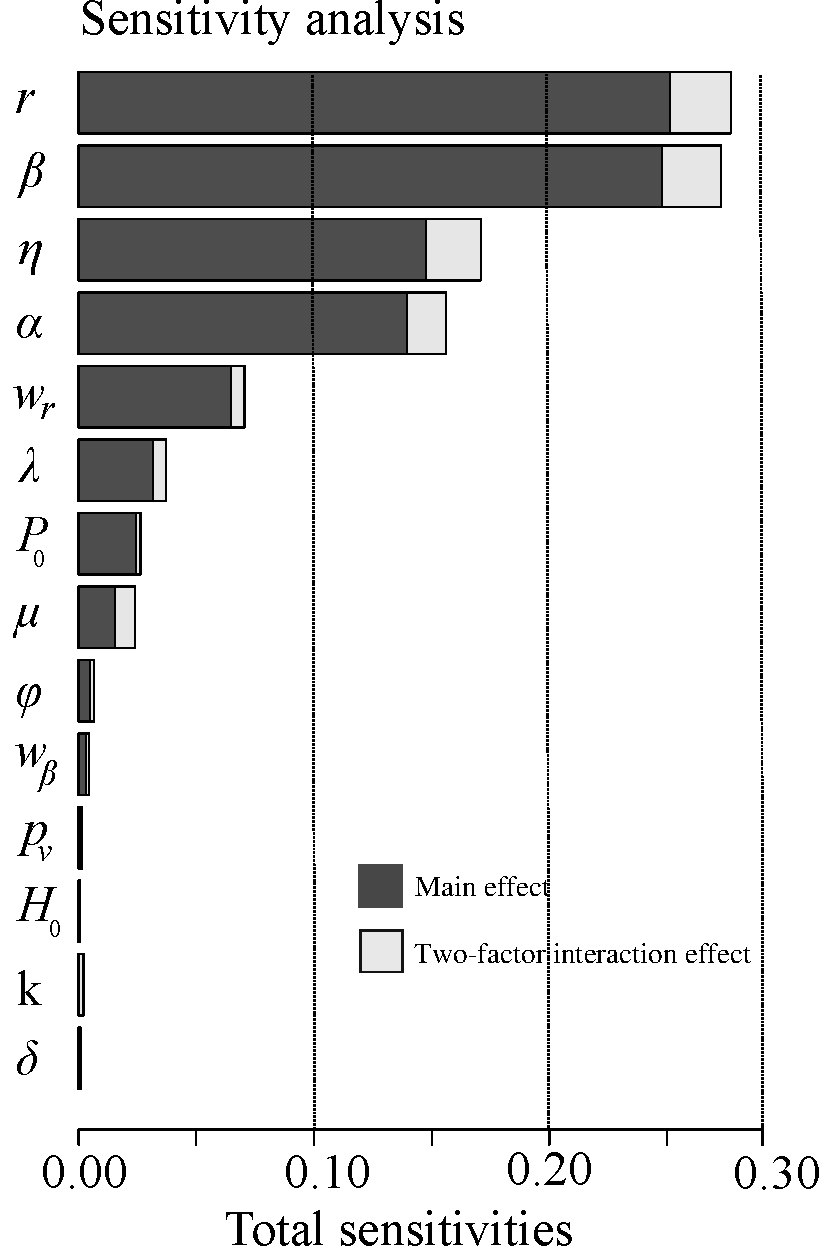
\includegraphics[width=.5\linewidth]{figS3.pdf}
  \caption[Global sensitivity indices on the performance for the optimal periodic rotation strategy over a 15-season time horizon]{Global sensitivity indices on the healthy root density ($\overline{HRD}$) for the optimal periodic rotation strategy over a 15-season time horizon.  Total sensitivity indices for the 14 parameters are ranked in descending order and split in main effect (black bar) and two-way interactions (grey bar) according to \eqref{si}.}
\label{figS3}
\end{figure}

